\section{Implementácia}

Aby fakultný robot dokázal využívať pohyby vypočítané inverznou kinematikou, opísané v kapitole \ref{sec_specification}, rozhodli sme sa výpočet, čo najviac oddeliť od súčasnej štruktúry kódu. Ako podklad sme si zvolili implementáciu diplomovej práce Pavla Meštaníka, ktorá je opísaná v kapitole \ref{sec_mestanik}. Vznikol tak samostatný balíček v jazyku Java s menom \texttt{sk.fiit.jim.agent.moves.ik}. 

Súčasťou sú tieto triedy:
\begin{itemize}
	\item \texttt{ForwardKinematicResult}
	\item \texttt{HeadIk}
	\item \texttt{Kinematics}
	\item \texttt{KinematicUtils}
	\item \texttt{LeftArmIk}
	\item \texttt{LeftLegIk}
	\item \texttt{Matrix}
	\item \texttt{Orientation}
	\item \texttt{RightArmIk}
	\item \texttt{RightLegIk}
	\item \texttt{SimsparkConstants}
\end{itemize}

Triedy \texttt{Kinematics}, \texttt{Matrix}, \texttt{Orientation} sú jediné, ktoré sú viditeľné aj v iných balíčkoch, ostatné sú viditeľné len v rámci nového balíka. V nasledujúcej kapitole \ref{sec_classes_desc} si popíšeme funkcionalitu každej triedy.

\subsection{Popis tried} \label{sec_classes_desc}
\textbf{Trieda \texttt{Kinematics}}
\\
Táto trieda obsahuje metódy, ktoré slúžia na vrátenie výsledkov výpočtov pre doprednú a inverznú kinematiku popísaných rovnicami z kapitoly \ref{sec_specification} pre všetky 4 končatiny (ľavú, resp. pravú ruku a ľavú, resp. pravú ruku). Výpočet pre hlavu sa momentálne nevyužíva.
\\\\
\textbf{Trieda \texttt{Matrix}}
\\
Slúži sa na maticové operácie, ktoré sa využívajú pri doprednej a inverznej kinematike. Zároveň obsahuje niektoré matice ako konštanty, ktoré sa často využívajú pri výpočtoch. 
\\\\
\textbf{Trieda \texttt{Orientation}}
\\
Úlohou tejto triedy je zapuzdriť natočenie koncového efektora podľa zodpovedajúcich osí $x$, $y$, $z$.
\\\\
\textbf{Triedy \texttt{LeftArmIk}, \texttt{LeftLegIk}, \texttt{RightArmIk}, \texttt{RightLegIk}, \texttt{HeadIk}}
\\
Obsahujú výpočty pre uhly zodpovedajúcim končatinám.
\\\\
\textbf{Triedy \texttt{SimsparkConstants}, \texttt{KinematicUtils}}
\\
Pomocné triedy na uchovávanie konštánt a pomocných metód pre všetky ostatné výpočty.
\\\\
\textbf{Ostatné triedy}
Zároveň boli rozšírené existujúce balíčky novými triedami. Tie slúžia na využije inverznej kinematike pri pohyboch robota. Nové triedy:
\begin{itemize}
	\item \texttt{DynamicMove} - slúži ako predloha pre dynamické pohyby pre \texttt{Ruby} triedy. Vstupom je sekvencia pozícií a natočení koncového vektora zodpovedajúcej končatiny.
	\item \texttt{RubyDynamicMove} - slúži na vytváranie sekvencií pozícií a natočení koncového efektora niektorej končatiny, teda vytvára pohyb.
	\item \texttt{PlanDynamicMove} - trieda pre plánovač, na využívanie dynamických pohybov.
\end{itemize}

Závislosti medzi triedami a balíčkami sú zobrazené na obrázku \ref{pic_class_diagram}. Obrázok neobsahuje všetky triedy, ale len relevantné pre opis implementácie. Novovytvorené triedy a balíčky sú zvýraznené tmavou farbou.

\begin{landscape}
\thispagestyle{empty}
\newgeometry{right=-8cm} % magické číslo, aby to bolo pekne zarovnané.
\begin{figure}[H]
\centering
	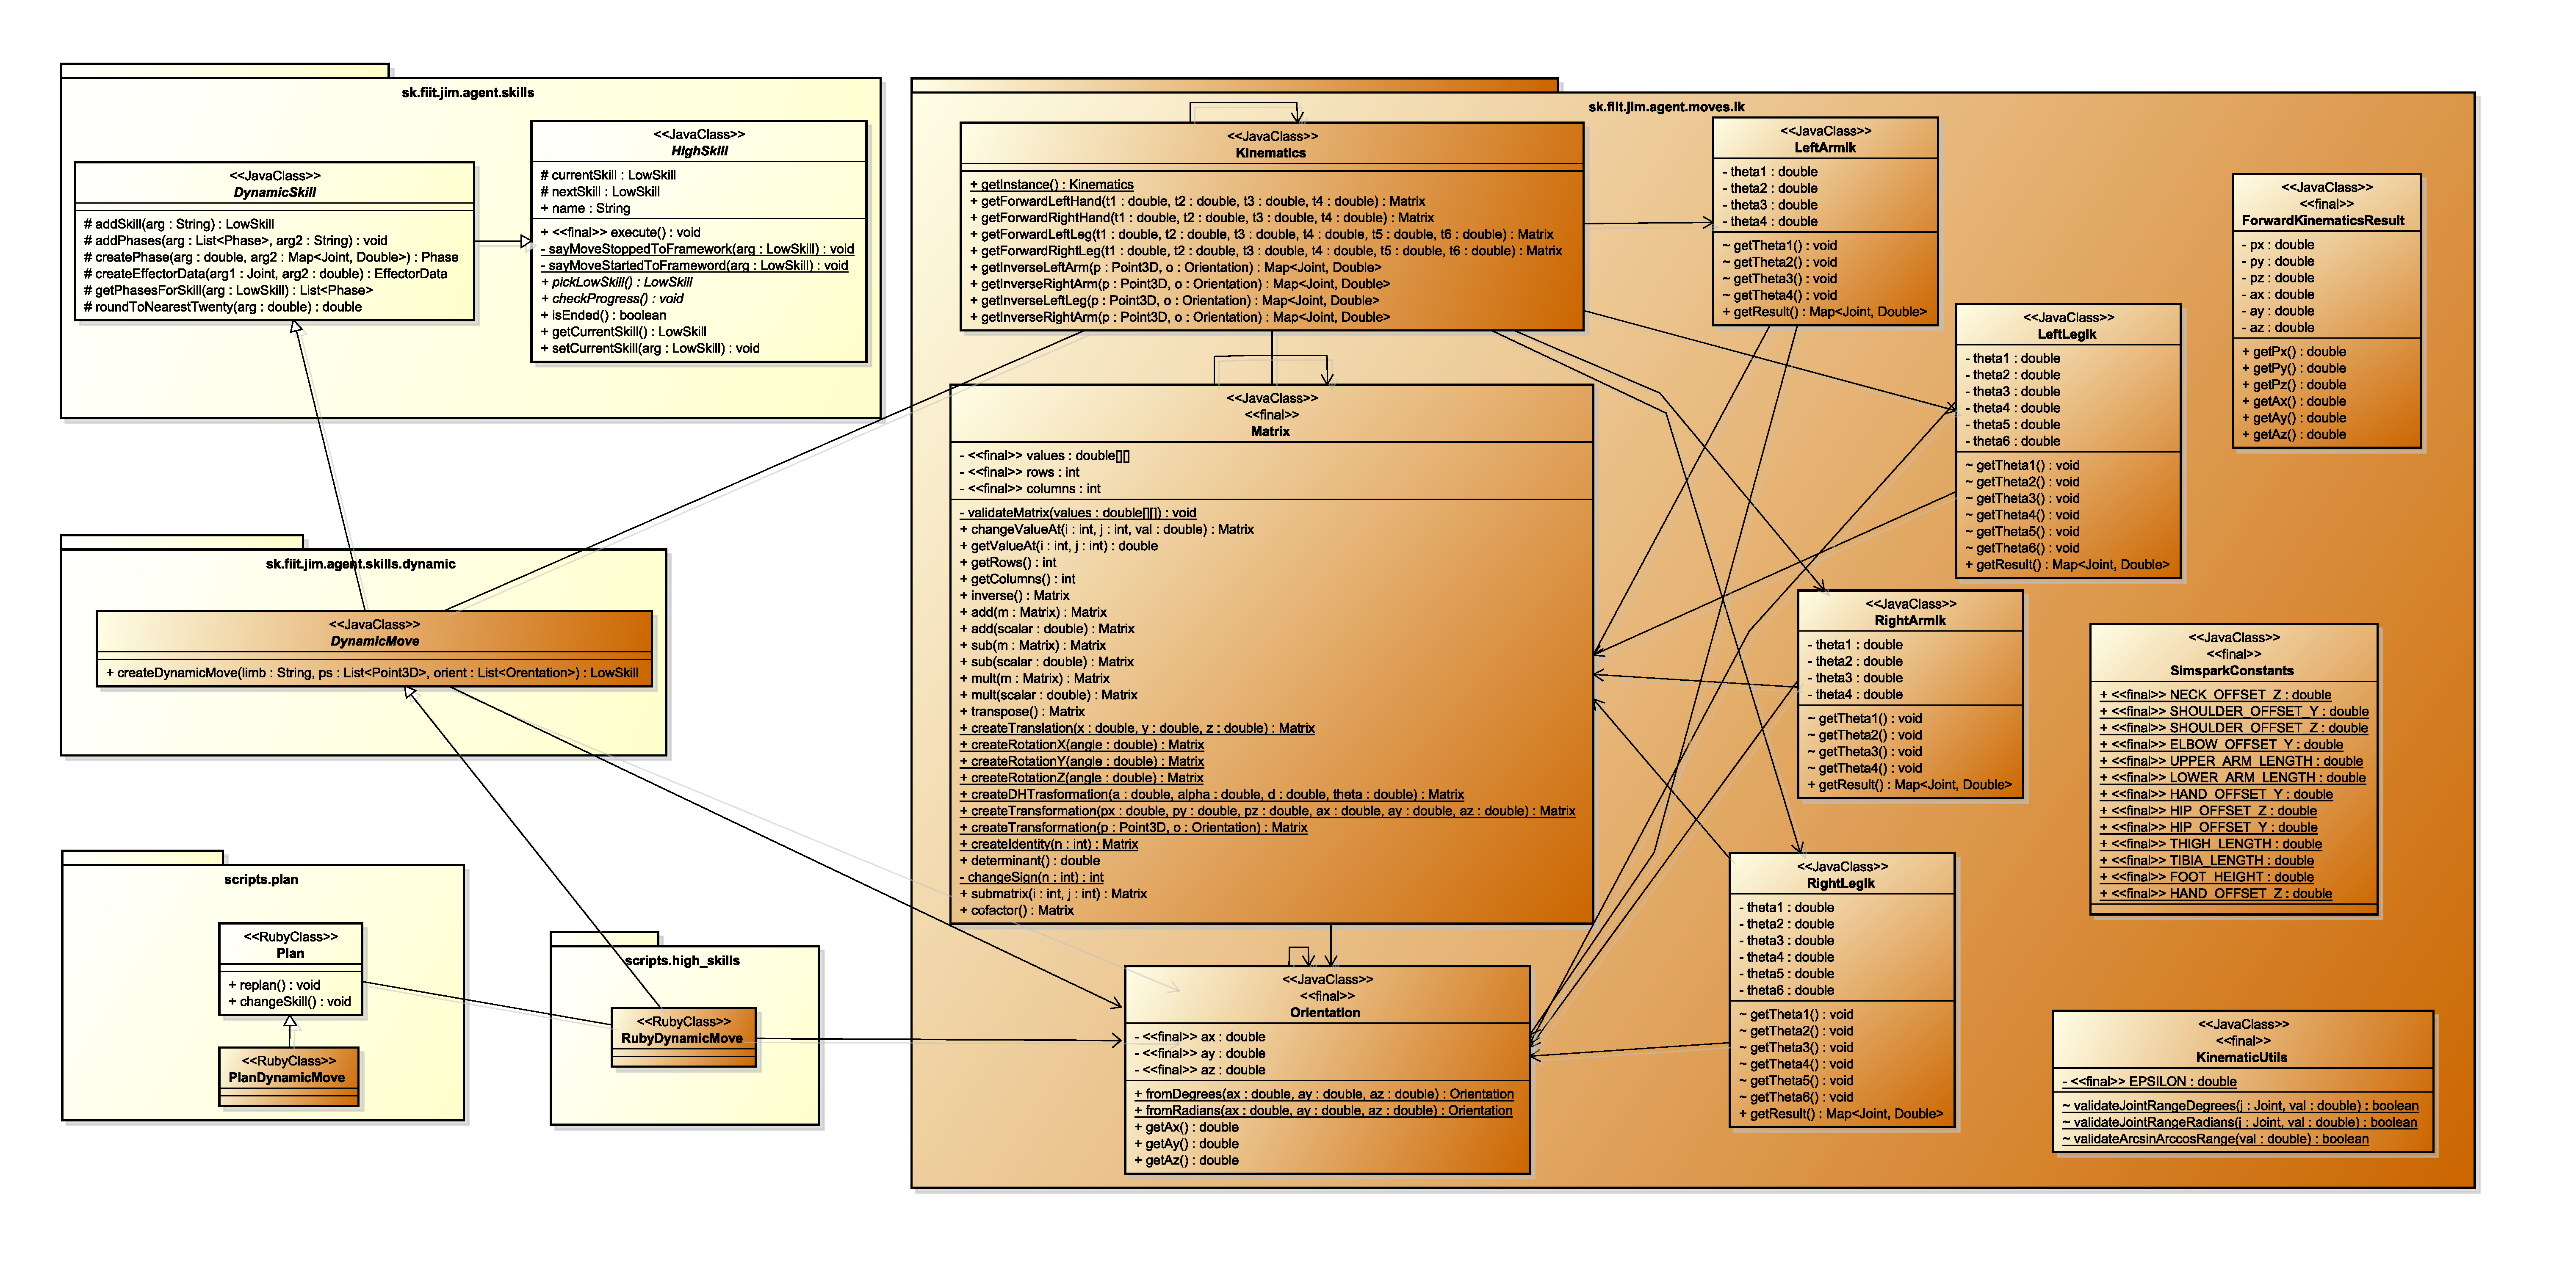
\includegraphics[scale=0.3]{./data/class_diagram}
	\caption{sdnaidna}
	\label{pic_class_diagram}
\end{figure}
\end{landscape}
